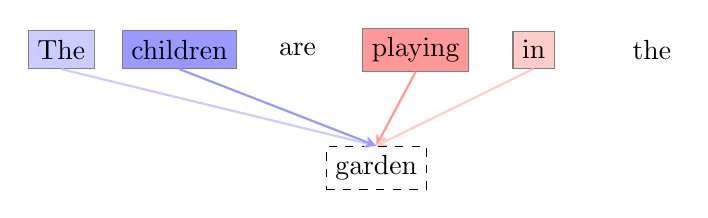
\begin{tikzpicture}[node distance=1.5cm]

% Define block styles
\tikzstyle{model} = [rectangle,rounded corners, minimum width=2cm, minimum height=1cm, text centered, draw=black, fill=blue!30]
\tikzstyle{arrow} = [thick,->,>=stealth]

% Define nodes
\node (the) [fill=blue!20,rectangle,draw=black!50] {The};
\node (children) [right of = the,fill=blue!40,rectangle,draw=black!50] {children};
\node (are) [right of = children] {are};
\node (playing) [right of = are,fill=red!40,rectangle,draw=black!50] {playing};
\node (in) [right of = playing,fill=red!20,rectangle,draw=black!50] {in};
\node (the2) [right of = in] {the};

\node (garden) [below of = are, xshift=1cm,rectangle,dashed,draw=black] {garden};

% Draw arrows
\draw [arrow,draw=blue!20] (the.south) -- (garden.north);
\draw [arrow,draw=blue!40] (children.south) -- (garden.north);
\draw [arrow,draw=red!40] (playing.south) -- (garden.north);
\draw [arrow,draw=red!20] (in.south) -- (garden.north);

% Add a rectangle around the last four nodes
\end{tikzpicture}